\documentclass[12pt]{article}

\usepackage{sbc-template}

\usepackage{graphicx,url}

\usepackage[brazil]{babel}   
%\usepackage[latin1]{inputenc}  
\usepackage[utf8]{inputenc}  
% UTF-8 encoding is recommended by ShareLaTex

     
\sloppy

\title{Construção de um ambiente virtual interativo utilizando técnicas de realidade Virtual com VRML}

\author{Fabio Vitor Noronha\inst{1}, Ewelly Fabiane de Sousa\inst{1}, Luciano Silva\inst{1}}


\address{Departamento de Ciência da Computação -- Universidade Federal de Roraima
  (UFRR)\\
  Boa Vista -- RR -- Brazil
  \email{fabio.vitor@ufrr.br, ewelly.sousa@ufrr.br,
  luciano.silva@ufrr.br}
}

\begin{document} 

\maketitle

\begin{abstract}
  This article presents a research project developed at the Federal University of Roraima (UFRR) with the objective of applying techniques and technologies for the reconstruction of UFRR campuses in virtual reality. Specifically, this article addresses the planning and construction of the science and technology block (CCT) using the VRML language.
\end{abstract}
     
\begin{resumo} 
  Este artigo apresenta um projeto de pesquisa desenvolvido na Universidade Federal de Roraima (UFRR) com o objetivo de aplicar técnicas e tecnologias para a reconstrução dos campi da UFRR em realidade virtual. Especificamente, este artigo aborda o planejamento e a construção do bloco de ciências e tecnologia (CCT) utilizando a linguagem VRML.
\end{resumo}


\section{Introdução}

Padrões como o VRML (\textit{Virtual Reality Modeling language}) e seu sucessor X3D (\textit{Extensible 3D}), por exemplo, têm sido a aplicados, entre outras coisas, para facilitar a visualização de conteúdos 3D na internet \cite{web3d2005open} e isso permite que usuários com conhecimentos limitados em sistemas de visualização tenham experiências de natureza multidimensional \cite{buriol2007modelagem}.

Nesse contexto, 




\begin{figure}[ht]
\centering
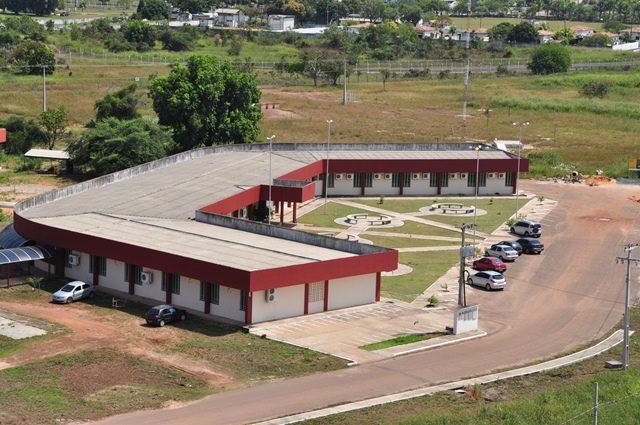
\includegraphics[width=.7\textwidth]{upper.jpg}
\caption{Visão superior do CCT}
\label{fig:upperviewblockv}
\end{figure}


\bibliographystyle{sbc}
\bibliography{sbc-template}

\end{document}
